\documentclass[a4paper,12pt]{article}
\usepackage{graphicx}
\usepackage{amsmath}
\usepackage{tkz-euclide}
\usepackage{booktabs}
\title{Assignment-4\\ Latex Report}
\author{Fuzayil Bin Afzal Mir}
\date{16/01/2021}
\begin{document}
	\maketitle
	
	
	\newpage
	\begin{itemize}
	    \item \Large\textbf{Exercise 2.9}
	\end{itemize}
	\section{Draw a $\triangle$ABC, given that a+b+c=11, $\angle$B = 30$^{\circ}$ and $\angle$C = 90$^{\circ}$}\\
    	
\subsection{Solution} \\

\textbf{Figure of triangle ABC}

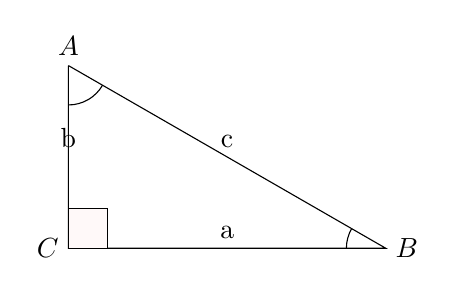
\begin{tikzpicture}[scale=1]
    \coordinate[label=right:$B$] (B) at (4.03,0);
    \coordinate[label=left:$C$] (C) at (0,0);
    \coordinate[label=above:$A$] (A) at (0,2.32);
    
    \draw (A)--node[above] {$\textrm{c}$}
    (B)--node[above] {$\textrm{a}$}
    (C)--node[above] {$\textrm{b}$}(A);
    \tkzMarkAngle[fill=green!15,size=0.5](C,A,B);
    
    \tkzMarkRightAngle[fill=pink!10,size=0.5](B,C,A);
    
     \tkzMarkAngle[fill=green!30,size=0.5](A,B,C);
    \end{tikzpicture}





It,s given that, \begin{equation}
    a+b+c=11
\end{equation}\\
and,\\

$\angle$B = 30$^{\circ}$ 
Now,
Sin(30$^{\circ}$ )= \dfrac{b}{c}\\

\dfrac{1}{2}=\dfrac{b}{c}\\

therefore,\\

\begin{equation}
  b=\dfrac{c}{2}  
\end{equation}\\


Also,
Cos(30$^{\circ}$ )= \dfrac{a}{c}\\

\dfrac{\sqrt{3}}{2}=\dfrac{a}{c}\\

therefore,\\
\begin{equation}
    a=\dfrac{c\sqrt{3}}{2}
\end{equation}\\

Now substituting the values of b and a in the equation (1).\\
we get,\\

\dfrac{c\sqrt{3}}{2}+\dfrac{c}{2}+c=11\\$$\\

\dfrac{c\sqrt{3}+c+2c}{2}=11\\$$\\

c\sqrt{3}+3c=22\\$$\\

c(3+\sqrt{3})=22\\$$\\

c= \dfrac{22}{3+\sqrt{3}}\\$$\\

c= \dfrac{22}{3+\sqrt{3}}* \dfrac{3-\sqrt{3}}{3-\sqrt{3}}\\$$\\

c=\dfrac{27.9}{6}\\

\begin{equation}
    c=4.65
\end{equation}\\

Now using value of c in equation(2) and equation(3)\\
we get,\\$$\\

a=\dfrac{4.65\sqrt{3}}{2}\\$$\\
a=4.03 \\
and,\\
b=2.32\\

hence we got,\\


\fbox{a=4.03}\\

\fbox{b=2.32}\\

\fbox{ c=4.65}\\

since sum of angles of a triangle is always equal to 180$^{\circ}$\\

therefore in the given Triangle,\\

$\angle$A+$\angle$B+$\angle$C=180$^{\circ}$\\

$\angle$A+30$^{\circ}$+90$^{\circ}$=180$^{\circ}$ \hspace{3cm}{[\angle$B=30$^{\circ}$ and $\angle$C=90$^{\circ}$}--given]\\

$\angle$A=180$^{\circ}$-120$^{\circ}$\\

\fbox{
$\angle$A=60$^{\circ}$}\\


\section{Steps Of Construction:}\\

1) Draw a line AB equal to the length of c=4.65\\

2) With A as centre draw an arc of length of b=2.32\\

3) With B as centre draw an arc of length a=4.03\\

4) Mark the point as C where two arcs meet each other.\\

5) Join C to A and C to B.\\

6)Hence ABC is the required triangle.\\

\subsection{Figure of Triangle ABC}

 \\
 


\newpage
\begin{center}
    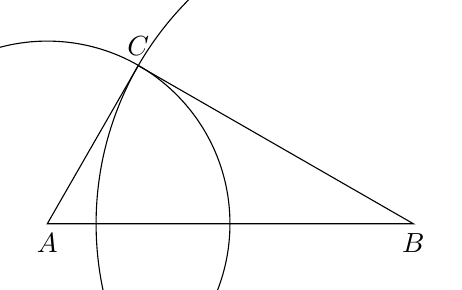
\begin{tikzpicture}[scale=1]
        \coordinate[label=below:$A$] (a) at (0,0);
        \coordinate[label=below:$B$] (b) at (4.65,0);
        \begin{pgfinterruptboundingbox}
            \node(Cric1) at (a) [draw,circle through=($ (a) + (0:2.32) $)] {};
            \node(Cric2) at (b) [draw,circle through=($ (b) + (0:4.03) $)] {};
        \end{pgfinterruptboundingbox}
        \coordinate[label=above:$C$] (c) at (intersection 2 of Cric1 and Cric2);
        \draw(a)--(c)--(b)--cycle;
        
    \end{tikzpicture}
\end{center}






















\end{document}
